% Created 2021-11-15 Mon 21:06
% Intended LaTeX compiler: pdflatex
\documentclass[11pt]{article}
\usepackage[utf8]{inputenc}
\usepackage[T1]{fontenc}
\usepackage{graphicx}
\usepackage{grffile}
\usepackage{longtable}
\usepackage{wrapfig}
\usepackage{rotating}
\usepackage[normalem]{ulem}
\usepackage{amsmath}
\usepackage{textcomp}
\usepackage{amssymb}
\usepackage{capt-of}
\usepackage{hyperref}
\author{Olivier Ma}
\date{\today}
\title{Probabilistic modelling in Python\\\medskip
\large With Pyro, PyTorch, and Limited Imagination}
\hypersetup{
 pdfauthor={Olivier Ma},
 pdftitle={Probabilistic modelling in Python},
 pdfkeywords={},
 pdfsubject={},
 pdfcreator={Emacs 27.2 (Org mode 9.4.6)}, 
 pdflang={English}}
\begin{document}

\maketitle
\tableofcontents


\section{Introduction to probability and modelling}
\label{sec:orgbbe43be}
In computer programs, everything is, in one way or another, represented as numbers. There are no cars, plants, cats or circus fools, there are only numbers. Similarly in probabilistic modelling there are only probability distributions. Observed visible variables, unobserved hidden variables, parameters, models, predicted quantities, everything has a distribution. (A word on the vocabulary here: the word "variable" has something specific in probability theory, but that's not what it means here. In this book we use it to simply mean "a quantity that varies", similar to what it means in computer science.) And since they are fundamentally the same thing - quantities with associated uncertainties - we'll also treat them the same way. This is the principle of probabilistic modelling that we'll follow throughout the book.

This also gives us a very clear boundary between what's inside our model and what's not: just observe whether there are uncertainties around a given quantity, and whether there are probability distributions associated with them: if they do, they are part of the model; and if they don't, they are external factors we use to build the models.

Many different names have been given to describe what's essentially the same thing: Bayesian statistics, inverse probability, probabilistic programming, Bayesian inference, and so on, and probabilistic modelling among them. In this book I have chosen "probabilistic modelling" to specifically refer to building models, and leave "Bayesian inference" to the computation we do on these models.

Considering that the whole book will be about probabilistic modelling, it's only fair that we begin it with an introduction of probability theory. Obviously we won't be able to systematically cover everything here: what we are aiming at is a new probabilistic perspective to modelling, and some foundational tools to help you get through this book. This beginning is a bit theoretic, but I'll keep it conversational; the good news is that the key ideas of probability theory are not many and what we need are even less. Nevertheless, remember that Bayesian statistics is hard, because thinking is hard; and because the real world, and by extension the data we'll be dealing with have complex relationships. 

We first import some libraries for visualisation, and we'll use the probability distributions implemented in PyTorch to illustrate the concepts we'are going to cover.

\begin{verbatim}
import torch
import torch.distributions as dist
import matplotlib.pyplot as plt
import seaborn as sns
\end{verbatim}

\subsection{A gentle introduction to probability theory}
\label{sec:org1f313bd}

A probability distribution is a systematic way to distribute probability. This might sound like tautology, but it's important to understand that the purpose of probability distributions is already clearly stated in its definition, The word "distribution" refers to an action of distributing things among certain recipients; here the thing being distributed is the probability mass, which always sums to 1, and the recipients are the elements in the probability space. In modern probability theory a probability distribution is usually defined as a triplet

$$(\mathbf{A}, \mathcal{A}, \mathbb{P}),$$

in which

\begin{itemize}
\item \(\mathbf{A}\) is a space, that is to say a collection of points;
\item \(\mathcal{A}\) is a sigma algebra defined on that space, that is a collection of well-behaving subsets of that space;
\item and \(\mathbb{P}\) is a Probability distribution, which is simply a function that maps the sets in a Sigma Algebra to points between \(0\) and \(1\).
\end{itemize}

To be a properly defined probability distribution, the mapping also has to satisfy three simple requirements:

\begin{itemize}
\item the probability assigned to the empty set is \(0\), i.e. \(\mathbb{P}(\phi)=0\),
\item the probability assigned to the whole set is \(1\), i.e. \(\mathbb{P}(\mathbf{A})=1\), and
\item for any two sets that have no intersections, the probability assigned to the union of the sets is the sum of the probabilities assigned to each of them, i.e. \(\mathbb{P}(S_1 + S_2) = \mathbb{P}(S_1) + \mathbb{P}(S_2)\).
\end{itemize}

That's it. It's a bit mouthful, it's terribly abstract, but fortunately we are done with it. (Spoiler alert: we are not. Its spectre will haunt us to the end of the book.) But before we go any further, let's first talk about why we'd want probability distributions in the first place, and then look at some simple examples.

There is no simpler probability distribution than the Bernoulli: its probability space has only two points, and one point less we will no longer be talking about probability, but certainty. The two points can be anything: whether it will rain tomorrow, whether to go to all tomorrow's parties, whether someone you are talking to on an internet forum is male or female, whether a nucleic test will turn out positive or negative, etc. It's an event with only two mutually exclusive outcomes.

For example, if we are talking about tomorrow's weather:

\begin{itemize}
\item the probability space: \(\{\text{rain}, \text{not rain} \}\)
\item the sigma-algebra: \(\{ \phi, \{\text{rain} \}, \{\text{not rain} \}, \{\text{rain}, \text{not rain} \} \}\)
\item the probability assignment: \(\mathbb{P}(\{\text{rain}\}) = p, \mathbb{P}(\{\text{not rain} \}) = 1- p\)
\end{itemize}

The empty set here can be understood as "nothing happens", there is no rain and there is no no rain; or that "everything happens", it's both raining and not raining; for sanity's sake it's understandable that we have assigned zero probability to it. It's worth Noticing that the probabilities are assigned to the sets, which are elements of the sigma algebra; not the events, which are elements of the space. But still, this is simple enough.

However problems begin to arise when we try to use numbers to indicate those events. It's common to use \(1\) to represent one of the events and \(0\) the other; it's equally common to use \(1\) for one and \(-1\) for the other; it's not at all common but equally acceptable to use \(1000000021\) for one and \(-4.281\) for the other.

But, if we look at these numbers, these numerical assignments are clearly not the same! The \((1, -1)\) pair has the heaven or hell dichotomy that gravitates, the \((1, 0)\) pair has the to be or not to be excitement that resonates, the \((1000000021, -4.281)\) pair has the inexplicable bizarreness that gnaws: how can they be the same? It turns out that all these differences are mere illusions, illusions forced upon us by the real numbers. The pun of reals and illusions are not intended, it's an unfortunate limitation of our language; and if we think about it, all puns are actually defaults of languages being put into entertainment use, with the confusion of the others as the dispense. The numerical differences are not present in the \((\text{rain, no rain})\) pair in our original problem, when we first built the probability distribution. The only thing matters in the numerical pairs are that they are different, how they differ does not matter; and if we try to do computations with the numbers themselves we'll be lost.

In statistical modelling we will, sooner or later, turn everything into numbers, but we should always keep in mind that numbers are only representations, not what things really are. The numerical representations are our tour guides in a new city, but they also have their own agenda: we need to rely on them because otherwise we'd be totally lost; but we should also be attentive to where they are leading us, lest they do things that will be detrimental to our own interest.

This is one of the most important reasons why when defining the probability distribution, we insist on using the very abstract notion of points, sets, spaces, and algebras. This system, albeit its obvious difficulty, is devised specifically for avoiding potential pitfalls like this, pitfalls we are likely to fall in if we start directly with the more familiar number system.

And before moving on, some observations worth being emphasised or reiterated:

\begin{itemize}
\item The probability distributed to the empty set is zero, but the probability of many non-empty sets can also be zero
\item Distributing the probability across a space is like distributing a million dollars to a crowd, you can choose however you want to distribute the money, but the sum is always fixed to one million. Besides, once the money is distributed, the amount of money everyone in the crowd has is fixed, there is no randomness in the distribution.
\item The probabilities are distributed to sets, that is the collections of points in the sigma algebra \(\mathcal{A}\), not to the points themselves in \(\mathbf{A}\). This is VERY important because points and sets have totally different properties. This has been the source of many confusion in practical application of probability theory, and also the source of many difficulty of probability computation.
\end{itemize}

\subsubsection{Constructing probability distributions}
\label{sec:org7e824e5}

We have discussed what probability distributions are, but we still need to figure out how to actually construct them. As we have seen, the formal definition of a probability distribution is quite abstract: one space, one sigma-algebra, one mapping between sets to numbers, and two or three rather simplistic rules. This is in sharp contrast to all the different distributions we might or might not have heard of, and the innumerable rules and relations of probability that we might or might not understand. So how do we actually build all the probability distributions? Based on how much information we have at hand, and how many assumptions we are willing to make, generally speaking we have several ways to do it, and we'll briefly introduce them here.

In the simplest case, all we have is a given space, and a sigma-algebra built on it, as defining a probability would demand. We know the properties of that space, and that of the sigma algebra, but we know nothing about the quantity we are modelling. Cautious modellers as we are, when we know nothing, we assume nothing. In this case we can just assign equal probabilities everywhere, which leads us to uniform distributions. These are not very interesting distributions, and neither are they particularly relevant to us, because when we want to model some quantity, we normally already have some ideas about it, no matter how vague these ideas might be. This leads us to the next scenario.

If, apart from the space and the sigma algebra, we also know some properties of the quantity we are modelling, then we might build some distributions that, by design, will meet these properties, while keeping the probability mass as normally distributed as possible. The properties under considerations normally include where the quantites concentrate, or how spreadout they are, and the principle we'll follow to build such distributions is called the principle of maximum entropy. Of course, the distributions built this way might not be, in the end, what we want, because even though they match some properties of the quantity we are modelling, they might fail to satisfy some other properties. So after having chosen a distribution based on some properties, it's always important to check whether the distribution also has other undesired properties. As we'll see in the future, this is an important part of probabilistic modelling.

If we already have one distribution defined on one space, with the holy triplet \((\mathbf{A}, \mathcal{A}, \mathbb{P})\) already in order, and we want to build a second distribution on a second space, then we might find some way to "transform" the first distribution on the first space to a second distribution on the second space. Understandably to do this we need to establish a mapping from points in the first space to the points in the second space. Probability distributions built this way are called transformed distributions, and you might be surprised to know that many of the distributions we know can be constructed this way. In the future, when we try to model some quantity that spread across some spaces where we don't have readily available distributions, this will be the method we will turn to.

After already having some simpler distributions defined on some simpler spaces, we can start treating them like Lego blocks, and assemble them together so that we can build other new distributions. This children's play is what will keep us busy for the rest of the book, since it's otherwise also known as probabilistic modelling.

In the rest of the book we'll encounter many different distributions; each time we meet a new one, it will be helpful to notice how it's been constructed, and whether there are other ways that we can achieve the same goal. Most distributions can be constructed in different ways, and these different ways often unveil different properties of the target distribution.

\subsection{The genesis}
\label{sec:orgf53bfaf}

If we just have a given space where we want to define a distribution, and we want the probability distribution to be as uniform as possible, the first choice, obviously, is the uniform distribution: no matter what the space is and how many points it contains, just assign each point set (a set containing one and only one point) the same probability value. However this is neither very practical nor very useful: if we want every point to have the same probability we wouldn't even need to define the probability in the first place! So instead we'll usually also enforce some extra requirements, like the average value of the distribution, or its variation across the whole space, or some other related quantities derived thereof, and we then contrive a scheme so that we can maximise the uniformness while at the same time preserving these requirements. This "uniformness" in probabilities are measured by something called the entropy, which is why these distributions are called maximum entropy distributions.

Depending on whether the probability space is discrete or continuous, we also give the schemes for probability assignments different names: probability mass functions if the space is discrete, and probability density functions if continuous. Undoutedly you have heard of these names somewhere already.

In this section we'll cover several maximum entropy distributions, which also happen to be the most widely used distributions in all probabilistic modelling. There are mainly two reasons for their popularity: they are mathematically simple and elegant, so they tend to be our first choices in modelling; they are able to describe the outcomes of many complex processes in real data problems, even when we know little about these complex processes, so they also tend to be our last choices.

\subsubsection{Bernoulli distribution}
\label{sec:org305d9b1}

Let's start with the Bernoulli distribution. We literally can not find any distribution simpler than the Bernoulli: it has only two possible outcomes, and one less will make it certainty, not probability. We assign probability \(p\) (\(0 \leq p \leq 1\)) to one of the outcomes and \((1-p)\) to the other, and if we take the possible outcomes \(b\) to be \(0\) and \(1\) (remember that this choice is completely random and in no way affects the actual distirbution assignment), the probability mass distribution can be written as

$$ \text{Bern}(b=1) = p, \text{Bern}(b=0)=1-p,$$

or in more succcint terms

$$ \text{Bern}(b; p) = p^b (1-p)^{1-b}.$$

We can easily verify that this probability assignment meets all the requirements of a probability distribution.

The mean and variance of the Bernoulli distribution are also easy to compute

\begin{align*}
\mathbb{E}(b) &= p \\
\mathbb{V}(b) &= p(1-p)
\end{align*}

\subsubsection{Beta distribution}
\label{sec:org18d26a0}

The Bernoulli distribution looks so simple that we didn't even bother to give any example. But think for a moment: we have assigned one outcome with probability \(p\) and the other \((1-p)\), but where is this mysterious \(p\) from? One day, you get up in the morning, you draw up the curtains, you see the clouds pressing on the window, and you wonder whether it's going to rain. Since you are not sure, you decide to assign it a probability, and this is where we need the Bernoulli distribution. However, not only you don't know whether it's going to rain, you also don't know how likely it's going to rain. That is, not only we don't know the \(b\) in \(\text{Bern}(b; p)\), we also don't know \(p\). Unlike \(b\), which can only take two values, \(p\) can be anything between \(0\) and \(1\). One probability distribution for such a space is the Beta distribution and since this space is continuous, the probability assignment is given by the probability density function.

The density for Beta distribuiton can be written as

$$\text{Beta}(p) \propto p^{a-1} (1-p)^{b-1}. $$

\(a\) and \(b\) are called the shape parameters and they can be any positive value, and the \(\propto\) reads "proportional to" and it simply means that I've taken the liberty to remove some clutter from the expression so that we can concentrate on things that matter. One day you might be interested in knowing what I have removed and it's alright, because the internet is just a few clicks away. we'll commit some similiar atrocities to some other distributions in the following text.

But for now, compare the density function of Beta with that of Bernoulli, you might be amazed to see how much they resemble each other. It turns out that the resemblence is intentional, and the intention is to make computation easier. Just looking at their expressions and we almost can't stop the urge to multiply them together. This conspiracy is called conjugacy, we won't touch on it much in this book but it used to be a great deal in Bayesian statistics.

There is a more general lesson to be learned here. In statistics, and more generally in all mathematics, everything is invented, for certain purposes, so when some formula is given to us, it's always a good idea to ask why they take the form as they are, and what purpose it serves.

One thing we might consider, when choosing probability distributions, is the shape of the probability density function, because it determines how much probability mass will be distributed to each area of the space. Look at the Beta density function, what shape do you think it will take? Let's take a closer look at the density function to see if we can find anything interesting.

The first thing we'll notice, is that the density function is the product of two functions, \(p^{a-1}\) and \((1-p)^{b-1}\), both are exponential functions, but since they have different signs (\(p\) and \(-p\)), they will probably move in opposite directions.

And, from our knowledge of exponential functions, we know that the functions have different behaviour when the exponential term is negative, smaller than one, and larger than one, which corresponds to \(a\) and \(b\) taking values smaller than 1, smaller than 2, and bigger than 2, respectively.

Let's plot the two functions separately, with different parameter values, to observe the function behavious under different conditions.

\begin{verbatim}
p = torch.arange(0, 1, step=0.01)
k0, k1, k2 = 0.8, 1.6, 4.8

fig, axs = plt.subplots(1, 2, figsize=(9, 4), sharey=True)

axs[0].plot(p, p**(k0-1), 'k-', label=f'k={k0}')
axs[0].plot(p, p**(k1-1), 'k--', label=f'k={k1}')
axs[0].plot(p, p**(k2-1), 'k:', label=f'k={k2}')
axs[0].legend()
axs[0].set_title(r'$p^{k-1}$')

axs[1].plot(p, (1-p)**(k0-1), 'k-', label=f'k={k0}')
axs[1].plot(p, (1-p)**(k1-1), 'k--', label=f'k={k1}')
axs[1].plot(p, (1-p)**(k2-1), 'k:', label=f'k={k2}')
axs[1].set_title(r'$(1-p)^{k-1}$')
axs[1].legend();
\end{verbatim}

\begin{center}
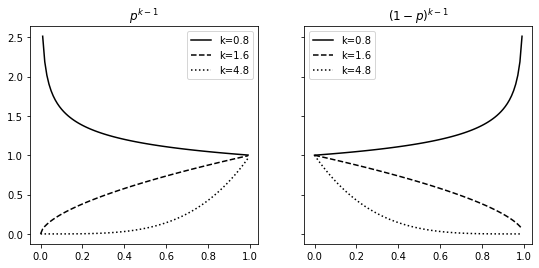
\includegraphics[width=.9\linewidth]{./.ob-jupyter/ab35f78f172dfab7dfd8bde3b1feccdc21ee89fc.png}
\end{center}

Because the plots on the left are about \(p\) while those on the right are about \(1-p\) it's understandable they have opposite shapes.
From the left plot, and together with a little knowledge about the exponential function, we see that

\begin{itemize}
\item when \(k<1\), the function is concave and decreases,
\item when \(1< k<2\), the function is convex and increases,
\item when \(k > 2\), the function is concave and increases.
\end{itemize}

The reverse is true for the plots on the right.
And now we can understand the shape of the Beta density functions, which are products of the two.

\begin{verbatim}
fig, axs = plt.subplots(2, 3, figsize=(9, 6), sharex=True)
axs = axs.flat

thetas = [(0.8, 0.8), (0.8, 1.6), (1.6, 4.8), (4.8, 4.8), (1.6, 0.8), (4.8, 1.6)]

for i, (a, b) in enumerate(thetas):
    d = dist.Beta(a, b)
    pdf = d.log_prob(p).exp()
    axs[i].plot(p, pdf, 'k-');
    axs[i].set_title('a={}, b={}'.format(a, b))
    plt.xticks([0, 0.5, 1])
    plt.tight_layout()
\end{verbatim}

\begin{center}
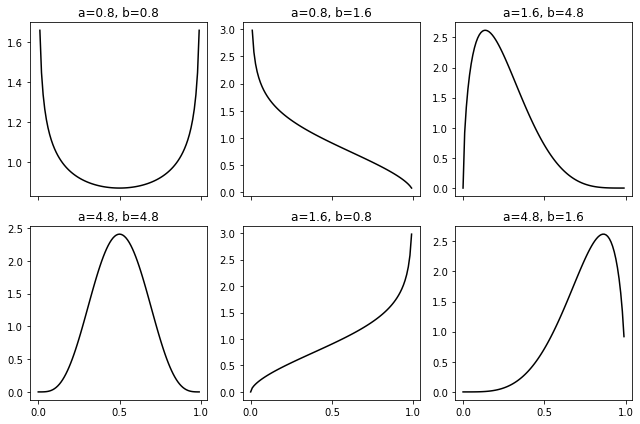
\includegraphics[width=.9\linewidth]{./.ob-jupyter/0aae13c28cf1a61c6aea2748c0539892205b758b.png}
\end{center}

From first impression we can already see that the density function is capable of taking many quite different shapes, even though the two components seem innocent enough.

\begin{itemize}
\item The upper left plot, where \(a<1, b<1\), is the product of the two green plots in the previous plot, the density is higher at the two extremes and lower in the middle
\item The bottom left plot, where \(a>1, b>1\), is the product of the two orange plots, the density is higher at the middle and lower at the two extremes.
\item The upper middle plot, where \(a<1, b>1\), is the product of the green on the left and orange on the right, so naturally it's monotonously decreasing
\item The lower middle plot, where \(a>1, b<1\), is the opposite
\item The upper right plot, where \(a>1, b>1\), is the product of the two green plots in the previous plot, the density is higher at the two extremes and lower in the middle
\item And although the two component functions and monotone, and product increases first and then decreases.
\item The upper right plot, where \(a\lt1, b\gt1\), is the product of two decreasing functions, the result is naturally a monotone decreasing function.
\item And further more, the exact values of \(a\) and \(b\) will determine how much the density increases before it starts decreasing.
\item The lower right is the opposite.
\end{itemize}

Studying the parameters and their effects on the density function can help us understand how the density functions are formed, and it also helps us to choose the right parameter values when we want a density function of a specific shape.

The mean and variance of the Beta distribution are

\begin{align*}
\mathbb{E}(p) &= \frac{a}{a+b} \\
\mathbb{V}(p) &= \frac{a}{a+b} \frac{b}{(a+b)(a+b+1)}
\end{align*}

It's a bit complex so let's remind ourselves the most important facts about them, before we move on and forget everything:

\begin{itemize}
\item the mean is a compromise between \(a\) and \(b\),
\item the variance is always smaller than the mean.
\end{itemize}

We have seen two probability distributions, and for both of them the variance is smaller than the mean. Is this a general rule? Well it's not, in the future we'll see many different distributions where the variance is equal to or greater than the mean. The lesson here, is that because these maximum entropy distributions are chosen for some of their properties, it's also important to check the others when we use these distribution to model some specific quantity.

\subsubsection{Gamma distribution}
\label{sec:org71565f2}

Sometimes life just feels like an endless struggle. We started with the Bernoulli distribution because all we want is an answer of yes or no, then we discovered that since we can not be sure, we have to think about the possibility of being yes or no, which is another quantity that can take any value between \(0\) and \(1\), and which we have patiently assigned a Beta distribution on. Then, to our utter exasperation, the Beta distribution itself have two more parameters and they can take on any values greater than 0. Does the struggle have no end?

I'm afraid the answer is: no, to live is to suffer, and there is no end. But lucky for us, both the parameters for the Beta distribution, \(a\) and \(b\), have the some domain, \(\mathbb{R}^+\), and we can thus put the same distribution on them.

A popular choice of probability distributions on this domain is the Gamma distribution, which itself has two parameters, the shape parameter \(\alpha\) and the scale parameter \(\beta\). Lucky for us, like \(a\) and \(b\) for the Beta distribution, \(\alpha\) and \(\beta\) have the same domain as them, \(\mathbb{R}^+\), so even if the worse has come to the worst and we also have to model \(\alpha\) and \(\beta\), we can just keep using the Gamma distribution. The density function for Gamma distribution is

$$\text{Gamma}(x; \alpha, \beta) \propto x^{\alpha-1} e^{-\beta x}. $$

Like the Beta density function, the Gamma density is the product of two functions; one of them is a geometric function \(x^{\alpha-1}\) just like Beta, and the other is an exponential function. Like before, let's plot out what these functions are like.

\begin{verbatim}
x = torch.arange(0.1, 10, step=0.1)
alphas = 0.8, 1.2
betas = 0.8, 1.6

fig, axs = plt.subplots(1, 2, figsize=(9, 4))

axs[0].plot(x, x**(alphas[0]-1), 'k-', label=f'alpha={alphas[0]}')
axs[0].plot(x, x**(alphas[1]-1), 'k--', label=f'alpha={alphas[1]}')
axs[0].legend()
axs[0].set_title(r'$x^{\alpha-1}$')

axs[1].plot(x, torch.exp(-1 * betas[0] * x), 'k-', label=f'beta={betas[0]}')
axs[1].plot(x, torch.exp(-1 * betas[1] * x), 'k--', label=f'beta={betas[1]}')
axs[1].set_title(r'$\exp{(-\beta x)}$')
axs[1].legend();
\end{verbatim}

\begin{center}
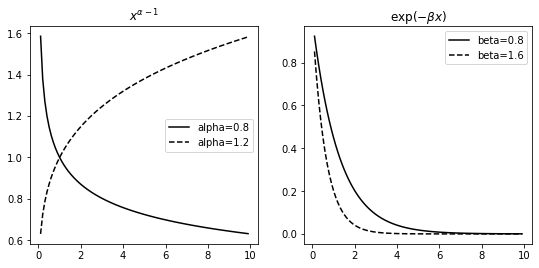
\includegraphics[width=.9\linewidth]{./.ob-jupyter/319aa3e48a825e567e7c63b0e68bdd3210ce6872.png}
\end{center}

When \(\alpha < 1\), the geometric function is strictly decreasing, when \(\alpha > 1\) it's strictly increasing; and for the exponential function, since it's actually a negative exponential function, it's always decreasing. The result of the interaction between the two functions, is that when \(\alpha < 1\) the density is always decreasing and when \(\alpha > 1\), it increases first and then starts decreasing. The value of \(\beta\) only changes the rate of change but not the overall shape of the distribution.

First let's fix \(\beta\) and see how \(\alpha\) affects the shape of the density.

\begin{verbatim}
alphas = [0.5, 2, 5]

fig, axs = plt.subplots(1, 3, figsize=(10, 4), sharex=True)
axs = axs.flat

for i, alpha in enumerate(alphas):
    d = dist.Gamma(alpha, 1)
    pdf = d.log_prob(x).exp()
    axs[i].plot(x, pdf, 'k-')
    axs[i].set_title('alpha={}, beta=1'.format(alpha))
    plt.xticks([0, 5, 10])
    plt.tight_layout();
\end{verbatim}

\begin{center}
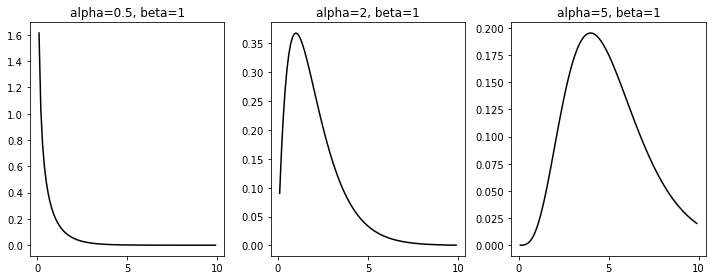
\includegraphics[width=.9\linewidth]{./.ob-jupyter/80083ecd858be97cb520fd66d7b81b26fd431aee.png}
\end{center}

As we can see, increasing \(\alpha\) gradually move the density towards the right. And this is why \(\alpha\) is called the shape parameter: it modifies the shape of the density function.

Now let's fix \(\alpha\) and see how changing \(\beta\) will change the shape of the density. It turns out that in PyTorch, and consequentially also in Pyro, the Gamma distribution is not parameterised with the scale parameter \(\beta\), but with another rate parameter \(\theta\). Fortunately there is a very simple relation between the two:

$$ \theta= 1 / \beta,$$

so converting from one to the other is quite easy.

\begin{verbatim}
x = torch.arange(0.1, 20, step=0.1)
betas = [0.5, 1, 2]

fig, axs = plt.subplots(1, 3, figsize=(9, 4), sharex=True, sharey=True)
axs = axs.flat

for i, beta in enumerate(betas):
    theta = 1 / beta
    d = dist.Gamma(2, theta)
    pdf = d.log_prob(x).exp()
    axs[i].plot(x, pdf, 'k-');
    axs[i].set_title('alpha=2, beta={}'.format(beta))
    plt.xticks([0, 5, 10, 20])
    plt.tight_layout()
\end{verbatim}

\begin{center}
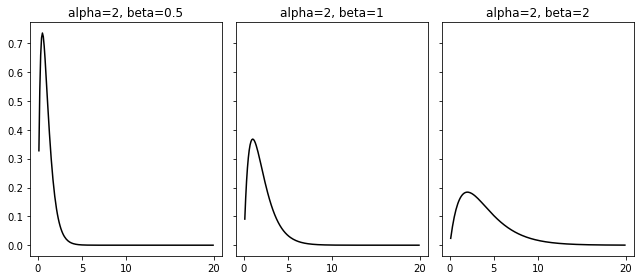
\includegraphics[width=.9\linewidth]{./.ob-jupyter/da4dfaf42c9ea90d5ed51f8892681df9f5722dde.png}
\end{center}

So \(\beta\) doesn't change the overall shape of the density function, it just stretches the density so it distributes the probability to wider areas. By the way that's why the parameter is called a "scale" parameter, because it scales the density function. It's inverse, \(\theta\), is called the rate parameter.

The mean and variance of the Gamma distribution are

\begin{align*}
\mathbb{E}(p) &= \frac{\alpha}{\beta} \\
\mathbb{V}(p) &= \frac{\alpha}{\beta^2}
\end{align*}

Depending on whether \(\beta\) is greater or smaller than 1, the variance can be samller or greater than the mean, so the Gamma distribution can be quite flexible in its shape. We like this, because this means that we can use the distribution in many different circumstances.

\begin{enumerate}
\item Exponential distribution
\label{sec:org5d59df0}

There are some special case Gamma distributions that are widely used in practice, here we'll mention one of them in passing, because we want to use it later.

The Gamma distribution is also called the exponential distribution when \(\alpha = 1\). We can understand why it's called exponential, because with \(\alpha=1\) the geometric part of the Gamma density disppears and we only have the exponential left. We can also guess the shape of the density function, because we have already plotted it when we were trying to understand the shape of the Gamma density function. It's also quite easy to get its mean and variance.

\begin{verbatim}
betas = [0.5, 2, 4]
x = torch.arange(0.1, 10, step=0.1)

fig, axs = plt.subplots(1, 3, figsize=(10, 4), sharex=True)
axs = axs.flat

for i, beta in enumerate(betas):
    d = dist.Gamma(1, 1/beta)
    pdf = d.log_prob(x).exp()
    axs[i].plot(x, pdf, 'k-')
    axs[i].set_title(r'$\beta$={}'.format(beta))
    plt.xticks([0, 5, 10])
    plt.tight_layout();
\end{verbatim}

\begin{center}
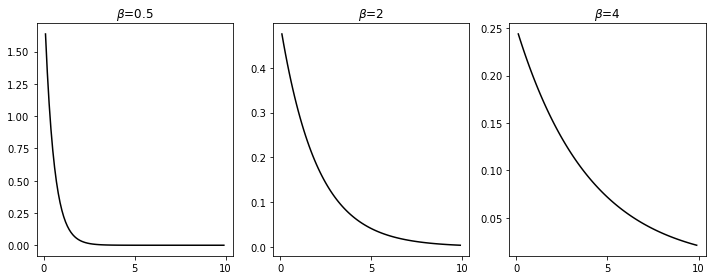
\includegraphics[width=.9\linewidth]{./.ob-jupyter/d3966c1d8501b2f112248d9cf12ad719b57d014a.png}
\end{center}

As we can see, scaling the distribution spreads the probability mass to wider regions, just like before.

There is another special case Gamma distribution, the Chi-squared distribution, that is one of the most important distributions in frequentist statistics, but we won't talk about it here.
\end{enumerate}
\subsubsection{Poisson distribution}
\label{sec:orgc69781d}

Now we come to the Poisson distribution, a distribution that is defined on the natural numbers. Actually, this sentence might give the wrong impression so let's start again: now we come to the space of natural numbers, and Poisson distribution is one maximum distribution defined on this space. It's always important to remember that when applying probability theory, we start with a quantity that we want to model, we study what space this quantity belongs to, then we search for probability distributions defined on this space. And since the natural numbers is a discrete space, we need its probability mass function:

$$\text{Pois}(n; \lambda) =  \frac{\lambda^n e^{-\lambda} }{n!}.$$

The Poisson distribution only has one rate parameter \(\lambda\), which, as it happens, is also the mean and the variance of the Poisson distribution.

Once the parameter value is fixed, the Poisson probability mass function only have two changing parts, the exponential term on the nominator, and the factorial term on the denominator. Clearly the factorial term is strictly increasing, and the exponential term is increasing when \(\lambda > 1\) and decreasing when \(\lambda < 1\), so for \(\lambda \leq 1\) we should see a decreasing mass function while for \(\lambda > 1\) the mass function should increase a while before it decreases. Let's plot out the mass function for different parameters and see how they looks like.

\begin{verbatim}
x = torch.arange(0, 20, step=1)
lbds = 0.5, 1, 5, 10

fig, axs = plt.subplots(1, 4, figsize=(9, 4), sharex=True, sharey=True)
axs = axs.flat

for i, lbd in enumerate(lbds):
    d = dist.Poisson(lbd)
    pdf = d.log_prob(x).exp()
    axs[i].plot(x, pdf, 'k-');
    axs[i].set_title(r'$\lambda={}$'.format(lbd))
    plt.xticks([0, 5, 10, 20])
    plt.tight_layout()
\end{verbatim}

\begin{center}
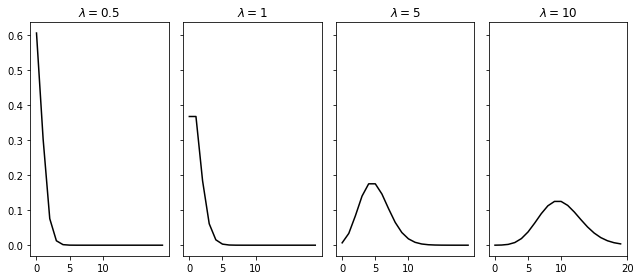
\includegraphics[width=.9\linewidth]{./.ob-jupyter/59dc2da23717c17b5ca70fd2f1a5a8138e0323d7.png}
\end{center}

Because the same parameter \(\lambda\) determines both the mean and the variance of the distribution, we can see that as \(\lambda\) grows the probability density is pushed more and more to the right while the variance also keeps increasing. Using one parameter to control both the mean and the variance makes the probability mass function formulation simple, but it also makes its application complicated since if the mean of the quantity we are modelling does not match the variance the distribution will become totally unusable. We'll come back to this problem later.

And still remember the Gamma distribution? We introduced it when we want a distribution for the shape parameters of the Beta distribution, whose domains are \(\mathbb{R}^+\). And since the rate parameter \(\lambda\) has the same domain, we can also put a Gamma distribution on it when necessary. In fact if the quantity modeled by the Gamma distribution is \(\lambda\) the Gamma density function can be written as

$$\text{Gamma}(\lambda; \alpha, \beta) \propto \lambda^{\alpha-1} e^{-\beta \lambda}. $$

If we ignore the factorial in the denominator of Poisson mass function, the two looks strikingly similar. That, of course, is the reason why Poisson and Gamma density function have similiar shapes, and the is also why we like to use the Gamma distribution to model \(\lambda\): it greatly simplifies the mathematical manipulation.

\subsubsection{Normal distribution}
\label{sec:orgd080ebe}

We are now arriving at the most important probability distribution in all of statistics, the Normal distribution. The Normal distribution is important mostly for two reasons:

\begin{itemize}
\item Because of the space it is defined on. The Normal distribution is a maximum entropy distribution on the real line, which happens to be the most important space in all of statistical modelling, and arguably in all of mathematics. Many of the quantities we want to study will be defined on the real line and even if they are not, the real line is a very good first approximation (and very often the last).
\item Because of a common theorem in probability theory, the Central Limit Theorem, which states that, under some common regularity conditions, if a quantity is the effect of multiple different causes added together, even if we have no idea what those causes are, the resulting effect tend to be Normally distributed. Since in statistics it's not uncommon to study things of whose causes we have little idea, the Central Limit Theorem and the Normal distribution offers us great confidence in blindly applying our hard learned statistics techniques.
\end{itemize}

The density function of the Normal distribution is an exponentiated square function:

$$\text{N}(x; \mu, \sigma) \propto \exp(- \frac{(x - \mu)^2}{2\sigma^2}).$$

The density function has two parameters, the mean \(\mu\), which can be any real value; the standard deviation \(\sigma\), which can only be positive. Let's plot out the density function, together with its two compoents: the square function and the exponential function.

\begin{verbatim}
mus = 0, 0
sigmas = 0.5, 1

fig, axs = plt.subplots(1, 3, figsize=(12, 4))

x = torch.arange(-20, 20, step=0.1)
axs[0].plot(x, -0.5 * (x-mus[0])**2 / sigmas[0]**2, 'k-',
            label=r'$\mu={}, \sigma={}$'.format(mus[0], sigmas[0]))
axs[0].plot(x, -0.5 * (x-mus[1])**2 / sigmas[1]**2, 'k--',
            label=r'$\mu={}, \sigma={}$'.format(mus[1], sigmas[1]))
axs[0].set_title(r'$- (x - \mu)^2/2\sigma^2$')

x = torch.arange(-10, 0, step=0.1)
axs[1].plot(x, torch.exp(x), 'k-',)
axs[1].set_title(r'$e^x$')

x = torch.arange(-5, 5, step=0.1)
axs[2].plot(x, torch.exp(-0.5 * (x-mus[0])**2 / sigmas[0]**2), 'k-',
            label=r'$\mu={}, \sigma={}$'.format(mus[0], sigmas[0]))
axs[2].plot(x, torch.exp(-0.5 * (x-mus[1])**2 / sigmas[1]**2), 'k--',
            label=r'$\mu={}, \sigma={}$'.format(mus[1], sigmas[1]))
axs[2].set_title(r'$\exp(- (x - \mu)^2/2\sigma^2)$')

handles, labels = axs[2].get_legend_handles_labels()
fig.legend(handles, labels, loc='center');
\end{verbatim}

\begin{center}
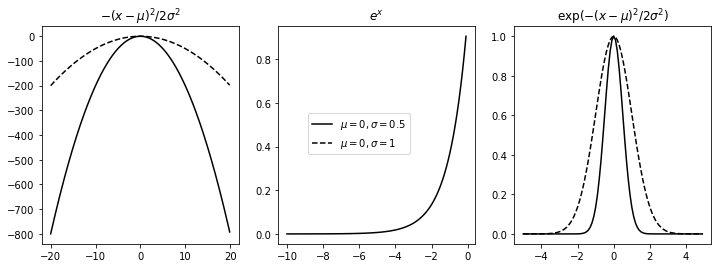
\includegraphics[width=.9\linewidth]{./.ob-jupyter/e38f535fecdb4c3e4283ca3f8f37e7246bc89b2b.png}
\end{center}

From the left plot we see that the negative square function is symmetric around \(\mu\), where it takes its maximum value \(0\), and it can take on huge negative values when \(x\) is far away from it. However, in the middle plot, we can see that when \(x\lt-5\), the exponential function is almost unresponsive to the input because the output is always close to zero. The combined effect of the two, as shown in the right plot, is that the density is very high around the mean, and it rapidly decreases when the input moves away from the mean. This combined effect guarantees that once the mean is decided, the majority of the probability mass will be around the mean, while the level of concentration will be determined by \(\sigma\). This is why we often see the adult hights or students' scores being modeled with the Normal distribution, even though we know perfectly well that their values will only appear on a very small region of the real line. We don't have to worry because the probabilition distribution scheme of the Normal distribution determines that we'll never wander very far from the mean, and this, let's be clear, is thanks to the shape of the exponential function.

As is already customary now, let's look at how the parameter values affect the shape of the density function. First \(\mu\).

\begin{verbatim}
x = torch.arange(-10, 10, step=0.1)
mus = -4, -1, 0, 3

fig, axs = plt.subplots(1, 4, figsize=(9, 4), sharex=True, sharey=True)
axs = axs.flat

for i, mu in enumerate(mus):
    d = dist.Normal(mu, 1)
    pdf = d.log_prob(x).exp()
    axs[i].axvline(x=0)
    axs[i].plot(x, pdf, 'k-')
    axs[i].set_title(r'$\mu={}$'.format(mu))
    plt.xticks([-10, 0, 10])
    plt.tight_layout();
\end{verbatim}

\begin{center}
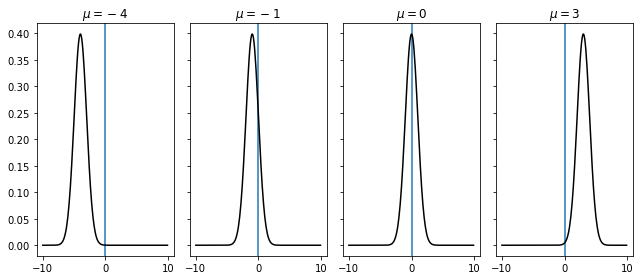
\includegraphics[width=.9\linewidth]{./.ob-jupyter/3ec562ebdc01c54f7f46570b41bbac3db8641c92.png}
\end{center}

Changing the mean does not change the shape of the distribution at all, it just moves the whole density function around the real line. Let's also look at \(\sigma\).

\begin{verbatim}
x = torch.arange(-10, 10, step=0.1)
sigmas = 0.5, 1, 2, 3

fig, axs = plt.subplots(1, 4, figsize=(9, 4), sharex=True, sharey=True)
axs = axs.flat

for i, sigma in enumerate(sigmas):
    d = dist.Normal(0, sigma)
    pdf = d.log_prob(x).exp()
    axs[i].plot(x, pdf, 'k-')
    axs[i].set_title(r'$\sigma={}$'.format(sigma))
    plt.xticks([-10, -5, 0, 5, 10])
    plt.tight_layout();
\end{verbatim}

\begin{center}
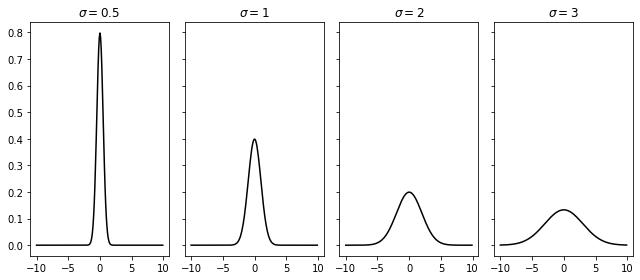
\includegraphics[width=.9\linewidth]{./.ob-jupyter/21dae2b6eb42c8486a45650ed198bfb1ed3e5650.png}
\end{center}


This time, changing \(\sigma\) does not seem to change the mean value at all, it just spreads the probabilition more widely when \(\sigma\) gets bigger. So the effect of \(\mu\) and \(\sigma\) are completely separated: the mean determines where the density will concentrate on while the standard deviation determines how much the probability spreads around it.

Of course this result shouldn't surprise anyone: anyone who has taken any elementary statistics class knows it, it's one of those things so banal that mentioning it is almost an offense. However, up to this point we have already studied several distributions and if we reflect on them a little bit, we'll realise that this is actually a quite rare property of the Normal density function, because for all the density functions we have covered so far, none of them has completely separated means and variances, and there is even the extreme case with the Poisson distribution, where the mean and the variance is always kept the same. So this property shouldn't be taken lightly.

And if we want to model the two parameters of the Normal distribution, we now also have enough distributions to do it. The domain of the mean parameter \(\mu\) is \(\mathbb{R}\), so we can put another Normal distribution on it; and the domain of the standard deviation parameter \(\sigma\) is \(\mathbb{R}^+\), so the Gamma distribution can come to the rescue. However, like we have already mentioned before, the domain of the quantity we are modelling is not the only criteria we use to choose distributions; we also have to check whether the other aspects of the distribution matches that of the quantity we are modelling.

The Normal distribution is, judging by the name, normal. That's why it's used in so many differenct circumstances. But there are some abnormal situations where we need some extraordinary distributions. The two distributions we are going to cover next, the Laplace distribution and the Cauchy distribution, are also defined on the real line but as we will see, each of them possesses some extraordinary features.

\begin{enumerate}
\item Laplace distribution
\label{sec:org7b078bd}

When we talked about the Normal distribution, we mentioned that the density of the probability distribuiton drops rapidly when we move away from the mean. It turns out that there is another distribution, although otherwise quite like the Normal distribution, drops its density even more rapidly than the Normal, and that is the Laplace distribution.

The density function of the Normal distribution is

$$\text{Laplace}(x; \mu, b) \propto \exp(- \frac{|x - \mu|}{b}),$$

in which \(\mu\) is the expected value and it is defined on \(\mathbb{R}\) like in the Normal case, and \(b\) is the positive scale parameter. It's easy to show its difference with the Normal distribution once we plot them together:

\begin{verbatim}
mu, sigma, b = 0, 1, 1

fig, axs = plt.subplots(1, 3, figsize=(12, 4))

x = torch.arange(-5, 5, step=0.1)
axs[0].plot(x, -0.5 * (x-mu)**2 / sigma**2, 'k-')
axs[0].plot(x, -1 * torch.abs(x-mu) / b, 'k--')

x = torch.arange(-10, 0, step=0.1)
axs[1].plot(x, torch.exp(x), 'k-')
axs[1].set_title('Comparing Laplace and Normal distribution')

x = torch.arange(-10, 10, step=0.1)
axs[2].plot(x, torch.exp(-0.5 * (x-mu)**2 / sigma**2), 'k-',
            label=r'Normal: $\mu={}, \sigma={}$'.format(mu, sigma))
axs[2].plot(x, torch.exp(-1 * torch.abs(x-mu) / b), 'k--',
            label=r'Laplace: $\mu={}, b={}$'.format(mu, b))

handles, labels = axs[2].get_legend_handles_labels()
fig.legend(handles, labels, loc='center');
\end{verbatim}

\begin{center}
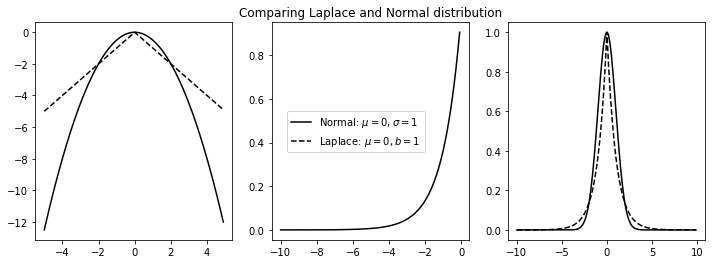
\includegraphics[width=.9\linewidth]{./.ob-jupyter/bf5d089d27ab646230a808172ae042fd88c00bfe.png}
\end{center}

We can clearly see where the difference is from. Both the functions being exponentiated are negative and symmetric around the mean, but in the Laplace case the function is linear while in the Normal case it's square. This causes the function is the Normal case to change more slowly around the mean and more rapidly when it's further away from the mean. Consequently, after passing through the exponential function, the resulting density function of the Normal distribution allocates more probability mass around the mean, but quickly reduces to close to zero when it's far away. The oppositive is true for the Laplace density function, it allocates less probability mass around the mean but when we moves away from the mean, it also decays alower.

This special property of the Laplace distribution makes it very helpful in certain circumstances, because it's exactly the oppositive of the Normal distribution. In practical statistical modelling the distribution is very often used to induce extreme behaviours: when the value is close to the mean we are much more likely to get the mean because the probability density is much smaller compared to the mean,but values far away from the mean are also acceptable because there are also considerable probability mass allocated to those regions.

The expected value of the Laplace distribution is \(\mu\), so changing \(\mu\) will change the central location of the density function; the variance of the distribution is \(2b^2\), which means that increasing \(b\) will cause the probability mass be spread out in wider regions, as shown in the next plot.

\begin{verbatim}
x = torch.arange(-10, 10, step=0.1)
bs = 0.5, 1, 2, 3

fig, axs = plt.subplots(1, 4, figsize=(9, 4), sharex=True, sharey=True)
axs = axs.flat

for i, b in enumerate(bs):
    d = dist.Laplace(0, b)
    pdf = d.log_prob(x).exp()
    axs[i].plot(x, pdf, 'k-')
    axs[i].set_title(r'$b={}$'.format(b))
    plt.xticks([-10, -5, 0, 5, 10])
    plt.tight_layout();
\end{verbatim}

\begin{center}
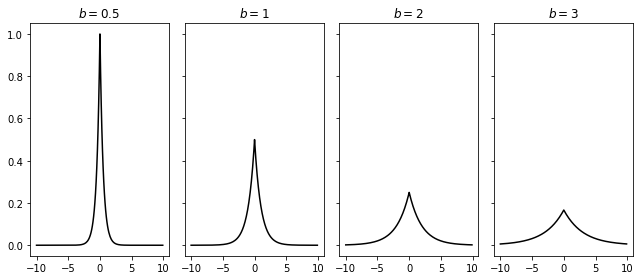
\includegraphics[width=.9\linewidth]{./.ob-jupyter/3747074d3c501a19cc66309cbec55f7aeaf4299c.png}
\end{center}

And, just in case you haven't notice it, the density function of the Laplace distribution is also a negative exponential function like the Exponential distribution, but with an extra absolute function so it's symmetrical around the mean. For this reason the Laplace distribution is also known as the Double Exponential distribution.

\item Cauchy distribution
\label{sec:orgf2acf09}

Now we already have two distributions defined on the real line:

\begin{itemize}
\item the Normal distribution, which limits the probability mass to a very
limited region around the mean
\item the Laplace distribution, which distributes less probability mass to
regions close to the mean and thus spreads the probability mass to
wider regions.
\end{itemize}

However, even though it's relatively heavy tailed compared to the Normal distribution, if we look at the Laplace density function, we can see that once beyond certain regions around the mean, there is hardly any probability mass left. If we truly want a heavy tailed distribution, a distribution that still has probability mass even when we are already far far away from the probability mass, then we need the Cauchy distribution. As a matter of fact the Cauchy distribution is so heavy tailed that we can't even properly defined its mean and variance, because any moment we can encounter a new extreme value that will totally derail our all previous computation of these characteristics.

The density function of the Cauchy distribution is

$$ \text{Cauchy} (x; x_0, \gamma) \propto { \gamma^2 \over (x - x_0)^2 + \gamma^2  }.$$

We have two parameters, the location parameter \(x_0\), whose domain is \(\mathbb{R}\); and the scale parameter \(\gamma\) whose domain is \(\mathbb{R}^+\). Again, we already have distributions defined on these domains, so we can model these extra quantities if we want.

As for the density function, we can see that we have a square function on the denominator

\begin{verbatim}
x0, gamma = 0, 1
fig, axs = plt.subplots(1, 3, figsize=(12, 4))

x = torch.arange(-5, 5, step=0.1)
axs[0].plot(x, (x-x0)**2, 'k-')
axs[0].set_title(r'$(x-x_0)^2$')

x = torch.arange(0, 25, step=0.1)
axs[1].plot(x, gamma**2 / (gamma**2 + x), 'k-')
axs[1].set_title(r'$\gamma^2 / (y + \gamma^2)$')

x = torch.arange(-10, 10, step=0.1)
axs[2].plot(x, gamma**2 / ((x-x0)**2 + gamma**2), 'k-')
axs[2].set_title(r'Cauchy density');
\end{verbatim}

\begin{center}
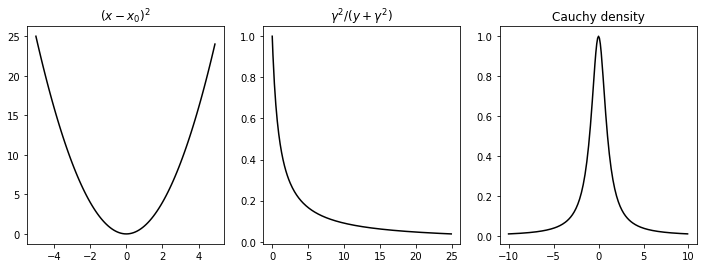
\includegraphics[width=.9\linewidth]{./.ob-jupyter/931278c6790dd7f9de71b96b7fb99a37dae25720.png}
\end{center}

The density function is symmetric: this is quite understandable since the square function is symmetric. On each side of the center, as we move away from \(x=x_0\), the square function on the left increases, the fraction function on the middle decreases, which leads to the decreasing density when we move away from the center, as shown in the right plot.

So where are the heavy tails coming from? Well clearly it's not from the square function because we are already using something similiar in the Normal distribution. If we compare the fraction function in the middle plot with the negative exponential functions we have seen before, we can clearly see that this function decreases as the exponential does, but at a much lower rate. In fact even in common language we use the word "exponential" quite often, to indicate how things change quickly, so it's understandable that the fraction function here doesn't change as fast as the exponential function. In any case this sluggish change means that even if we have moved fairly far away from the center, the density function would still be able to assign considerable probability mass in its vicinity. And this, is how we have succeeded in obtaining our heavy tail Cauchy distribution.

It's quite clear that the parameter \(x_0\) determines the center of the density function, but let's see how the density changes when we have different scale, \(\gamma\).

\begin{verbatim}
x = torch.arange(-10, 10, step=0.1)
bs = 0.5, 1, 2, 3

fig, axs = plt.subplots(1, 4, figsize=(9, 4), sharex=True, sharey=True)
axs = axs.flat

for i, b in enumerate(bs):
    d = dist.Cauchy(0, b)
    pdf = d.log_prob(x).exp()
    axs[i].plot(x, pdf, 'k-')
    axs[i].set_title(r'$\gamma={}$'.format(b))
    plt.xticks([-10, -5, 0, 5, 10])
    plt.tight_layout();
\end{verbatim}

\begin{center}
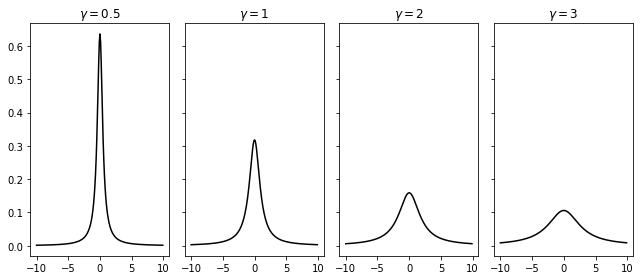
\includegraphics[width=.9\linewidth]{./.ob-jupyter/a8734fc48b326adc9fec6deceb27c7a13207522b.png}
\end{center}

Just as we suspected, scaling (i.e. increasing the scale parameter) spreads the probability mass to wider regions but it have no effect on the center of the distribution.

Up till now we have covered eight distributions on five different spaces:

\begin{itemize}
\item the Bernoulli distribution for a space with only two points;
\item the Poisson distribution for the natural numbers;
\item the Beta distribution for a section of the real line, \([0, 1]\), which is bounded on both sides;
\item the Gamma distribution for another section of the real line, \([0, +\infty]\) , which is bounded on one side, and its special case Exponential distribution;
\item the Normal distribution for the whole real line, and its Laplace and Cauchy variants with growing heavy tails.
\end{itemize}

At the end of this section, it's beneficial to remind ourselves what we are doing. We started with a certain space where we want to define a distribution, we then proceed to find a probability distribution that has maximum uniformity, because we don't have information on the quantity we are modelling and we don't want to pretend otherwise. But if we simply maximise the uniformity without any restrictions, we end up with uniform distributions everywhere, which is not what we want. So instead, we generally apply some restrictions to the maximising problem, normally restrictions about the center of the distribution, or its variation. And the distributions we have covered in this section are the outcomes of this maximisation process. We didn't specifically name the miximisation constraints because if we do, we'd also need to expalin exactly what maximisation we are doing, and that would get us into too much mathematical detail than I intended here.

Although not many, we have already covered some of the most important spaces, and some distributions defined on them; this will be the foundation on which we'll build the rest of the book.
\end{enumerate}

\subsection{The transformers}
\label{sec:org426b318}

We have already learned several different probability spaces and some probability distributions defined on them, but it's clear that these are not the only spaces we need in probabilistic modellings, and on those spaces, these probability distributions are not the only distributions we need. So how should we expand our arsenal of probability distributions?

After having already gone through the trouble of defining distributions only from first principles (i.e. principle of maximum entropy), we can now save some effort, and define new distributions by transforming the ones we already have. This is much easier than creating new distributions from scratch, and distributions created this way will also be easier for us to understand, since we already know the distributions they are generated from.

When constructing the probability distributions in the last section, we have taken great effort to explain how each of the density functions come about. This helps us to better understand the properties of the density functions, and this has also shown us the usefulness of using simple mathematical functions to achieve probability assignment goals. We have already seen that most density functions are constructed by combining some simple functions. Here we'll continue to do the same: we transform existing distributions with the help of some simple functions.

Very often in statistics we model quantities using some simple functions, like the linear functions, that will have outputs on the real line. These methods are called linear methods and are the most commonly used methods in all of statistics. Most of the transformations we will study in this section transforms a probability distribution defined on the real line to a part of it, and thus generalised the linear methods to many new problems.

\subsubsection{Trancation}
\label{sec:org6061c74}

Trancation is the simplest kind of transformation: after we've defined a distribution on a larger space, if we want a new distribution on a smaller space, we can simply throw away the redundant probability space and the probability mass distributed on it, and adjust accordingly the probability distribution on the remaining space so that it still sums up to \(1\).

Trancation happens when we want the properties of a certain probability density function, often how the probability is distributed around the mode or in the tails, but on a smaller space.

The most commonly used trancated distributions in probabilistic modelling are the Half Normal distribution and the Half Cauchy distribution, both of which throw away half of the probability distribution and keep the other half. And since most of the time the Trancated distributions are also centered at zero, so the new distributions are defined on the postive half of the real line, \(\mathbb{R}^+\).

Here is a comparison between the Normal distribution and the Half Normal distribution:

\begin{verbatim}
x0 = torch.arange(0.1, 5, step=0.1)
d0 = dist.HalfNormal(1)
pdf0 = d0.log_prob(x0).exp()
plt.plot(x0, pdf0, 'k--', label='Half Normal')

x1 = torch.arange(-5, 5, step=0.1)
d1 = dist.Normal(0, 1)
pdf = d1.log_prob(x1).exp()
plt.plot(x1, pdf, 'k:', label='Normal')

x2 = torch.arange(0.1, 5, step=0.1)
d2 = dist.HalfNormal(1)
pdf2 = d2.log_prob(x2).exp() / 2
plt.plot(x2, pdf2, 'k-', label='Half Normal, unnormalised')
plt.legend()
plt.title('Compare Normal and Half Normal distribution')
plt.tight_layout();
\end{verbatim}

\begin{center}
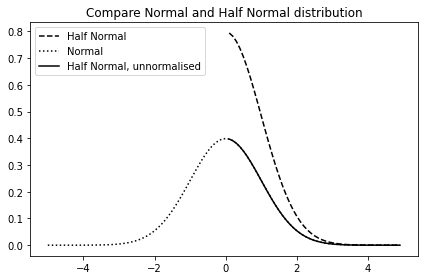
\includegraphics[width=.9\linewidth]{./.ob-jupyter/e79ea18b3b121c1d5e2c60e3f686534e3507d19c.png}
\end{center}


Before normalisation, the Half Normal distribution is, just as the name indicates, half of the Normal distribution. However since the probability mass for any probability distribution should sum to 1, we simply double the probability density at each point.

We expect the situation will be similiar with the Half Cauchy distribution:

\begin{verbatim}
x0 = torch.arange(0.1, 5, step=0.1)
d0 = dist.HalfCauchy(1)
pdf0 = d0.log_prob(x0).exp()
plt.plot(x0, pdf0, 'k--', label='Half Cauchy')

x1 = torch.arange(-5, 5, step=0.1)
d1 = dist.Cauchy(0, 1)
pdf = d1.log_prob(x1).exp()
plt.plot(x1, pdf, 'k:', label='Cauchy')

x2 = torch.arange(0.1, 5, step=0.1)
d2 = dist.HalfCauchy(1)
pdf2 = d2.log_prob(x2).exp() / 2
plt.plot(x2, pdf2, 'k-', label='Half Cauchy, unnormalised')
plt.legend()
plt.title('Compare Cauchy and Half Cauchy distribution')
plt.tight_layout();
\end{verbatim}

\begin{center}
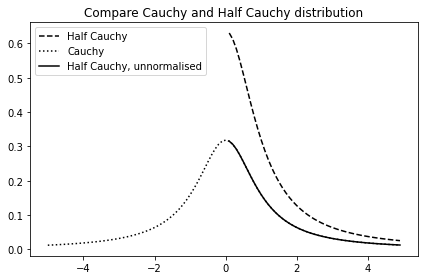
\includegraphics[width=.9\linewidth]{./.ob-jupyter/9261b5c1d61cb1e776c0d3f3bc040ab5922c2f00.png}
\end{center}

Just like the Normal case, only with heavier tails, as is characteristic of the Cauchy distribution.

There is of course no need to define a Half Laplace distribution since we already have the Exponential distribution.

Trancation at zero is obviously not the only way to trancate a distribution, but it's the most common case.

\subsubsection{Location-Scale transformation}
\label{sec:org04fe9f3}

We have seen in the previous section that many probability distributions are defined using a location parameter, which determines the center of the distribution, and a scale parameter, which determines how much the probability mass is spread around the center. It turns out that very often we can define a "standard" version of a distribution, often centered at \(0\) and with scale \(1\), and obtain other distribution by moving the center around or rescaling it. This is what's called the location-scale transformation.

The location-scale transformation is most often used on the Normal distribution. If we have already defined one Normal distribution, we can very easily define another using this transformation. The starting Normal distribution is often the Standard Normal, which is a Normal distribution with mean 0 and variance 1, but it can also be any other Normal distribution.

A Standard Normal distribution is defined as

$$x \sim \text{Normal} (0, 1),$$

then if we scale it with \(\sigma\) and add to it an extra constant \(\mu\) the resulting quantity

$$y = \mu + \sigma x$$

will have distribution

$$y \sim \text{Normal} (\mu, \sigma).$$

\begin{verbatim}
mu, sigma = 1, 2
fig, ax = plt.subplots()

x = torch.arange(-10, 10, step=0.2)
d0 = dist.Normal(0, 1)
pdf0 = d0.log_prob(x).exp()

x_samples = d0.sample([10000])
y_samples = mu + sigma * x_samples

d1 = dist.Normal(mu, sigma)
pdf1 = d1.log_prob(x).exp()

sns.histplot(y_samples, ax=ax, label=r'$y = {} + {} x$'.format(mu, sigma), stat='density', alpha=0.5)
plt.plot(x, pdf0, 'k-', label=r'$x \sim $ Normal(0, 1)')
plt.plot(x, pdf1, 'k--', label=r'$y \sim $ Normal({}, {})'.format(mu, sigma))

plt.xticks([-10, -5, 0, 5, 10])
plt.title('Loc-Scale transformation of Normal distribution')
plt.legend();
\end{verbatim}

\begin{center}
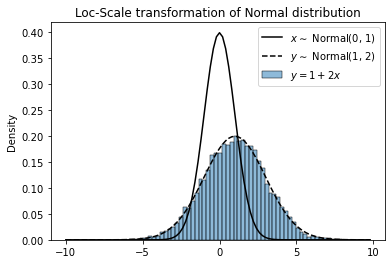
\includegraphics[width=.9\linewidth]{./.ob-jupyter/e92731eabdda0753d40e5c70ada87f191cb780c6.png}
\end{center}

The loc-scale transformation is very widely used on the Normal distribution, and considering how omnipresent the Normal distribution is in statistics, it's also one of the most commonly used transformation everywhere. This transformation is helpful because very often we want more than just modelling an unknown quantity with the Normal distribution; since we are also unsure about the mean and standard deviation of this quantity, we might want to model them as well. The location-scale transformation let us model them separately, and thus reduce the cognitive load for us and the computational load for the computers.

However we can't simply apply this transformation to whatever distribution we like: the distribution should first be defined by meaningful location and scale parameters. Besides there is something particular about the Normal distribution that makes this transformation especially useful, and that is the total separation between the mean and the variance. With the Normal distribution the \(\mu\) parameter controls the mean, the \(\sigma\) parameter controls the variance, and the two function separately without interfering with each other. This is a rare property of the Normal distribution that many other distributions don't have.

For example, suppose that we have a Gamma distributed quantity \(x\) with

$$x \sim \text{Gamma} (2, 1), $$

and we want an equally Gamma distributed quantity \(y\), with different parameters

$$y \sim \text{Gamma} (1.5, 1.2), $$

How can we apply the same location-scale transformation to achieve this? There is no obvious way to do it, because changing the mean will also affect the variance, and vice versa. However since the Gamma distribution has a scale parameter, we can scale it rather easily. For example we can scale \(x \sim \text{Gamma} (2, 1)\) to \(y \sim \text{Gamma} (2, 2.4)\) by simply using \(y = 2.4 x:\)

\begin{verbatim}
alpha, beta = 2, 2.4
fig, axes = plt.subplots(1, 1)

x = torch.arange(0.01, 15, step=0.1)
d0 = dist.Gamma(alpha, 1)
pdf0 = d0.log_prob(x).exp()

x_samples = d0.sample([10000])
y_samples = beta * x_samples

d1 = dist.Gamma(alpha, 1/beta)
pdf1 = d1.log_prob(x).exp()

sns.histplot(y_samples, ax=axes, stat='density', alpha=0.5)
axes.plot(x, pdf0, 'k-', label=r'x$\sim$ Gamma(2,1)')
axes.plot(x, pdf1, 'k--', label=r'y$\sim$ Gamma(2,2.4)')
axes.set_xlim([0, 15])
axes.set_title('Scaling the Gamma distribution')

plt.legend()
plt.xticks([0, 5, 10, 15])
plt.tight_layout();
\end{verbatim}

\begin{center}
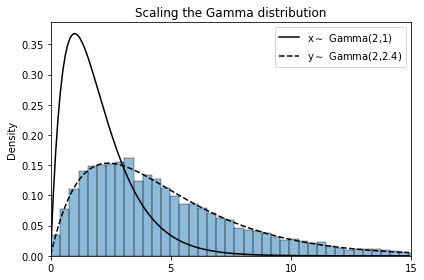
\includegraphics[width=.9\linewidth]{./.ob-jupyter/59bd25ca19d90e1a44996d15355d8ece74116224.png}
\end{center}

\subsubsection{Exponential transformation}
\label{sec:orgf10cbde}

We said in the previous section that it's important to understand how a distribution is constructed, so that we can know what further transformations are availabe to us. However this caution is only necessary if we want to maintain in the same family of distributions. In some other scenarios, if we just want to transform one distribution defined on one space to another distribution on a target space, without worrying about what the ending result is like, then this caution is not totally necessary. For example, if we simply want to transform a distribution defined on \(\mathbb{R}\) to another one defined on \(\mathbb{R}^+\), we can pass the original quantity through the exponential function without worrying about what the result distribution will be like, we are certain that the resulting distribution will have support on \(\mathbb{R}^+\). This is simply the property of the exponential function.

However a word of caution is needed here. Just because it's not necessary don't mean it's not beneficial. Transforming a distribution to another one in the same family has the benefit that we understand the properties of the new distribution; if we simply pass the quantity through some function, there is no guarantee what property the resulting probability distribution would have. In practice this can cause many unexpected modelling problems if we are not careful.

Here as a demonstration we'll pass a Normally distributed quantity through an exponential function:

$$ y = e^x.$$

\begin{verbatim}
fig, axes = plt.subplots(2, 1, figsize=(6, 6))

d0 = dist.Normal(0, 1)
x_samples = d0.sample([10000])
y_samples = x_samples.exp()

sns.histplot(x_samples, ax=axes[0], stat='density')
axes[0].set_xlim([-5, 5])

sns.histplot(y_samples, ax=axes[1], stat='density')
axes[1].set_xlim([0, 20])
axes[1].set_xticks([0, 5, 10, 15, 20])

plt.tight_layout();
\end{verbatim}

\begin{center}
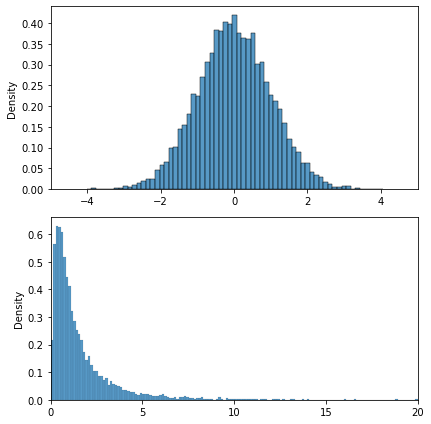
\includegraphics[width=.9\linewidth]{./.ob-jupyter/1367594e276ee8e864c489e0229ae01fb8100d18.png}
\end{center}

In this case we do know what the resulting distribution is: it's the LogNormal distribution, which is defined exactly as the exponential of a Normal distribution. However in general the resulting distribution doesn't have to correspond to any known distribution: this is where we can make use of our creativity, and where we need to assume the responsibility of being a responsible modeler.

We can also look at the distributions from a different perspective to gain some different insights on how the transformation works:

\begin{verbatim}
fig, axes = plt.subplots(3, 1, figsize=(6, 9))

d0 = dist.Normal(0, 1)
x_samples = d0.sample([10000])
y_samples = x_samples.exp()

for i in range(len(x_samples)):
    x, y = x_samples[i], y_samples[i]
    if x < 0:
        axes[0].axvline(x, color='k', alpha=0.01)
        axes[2].axvline(y, color='k', alpha=0.01)
    elif x < 1:
        axes[0].axvline(x, color='k', alpha=0.01)
        axes[2].axvline(y, color='k', alpha=0.01)
    elif x < 2:
        axes[0].axvline(x, color='k', alpha=0.01)
        axes[2].axvline(y, color='k', alpha=0.01)
    else:
        axes[0].axvline(x, color='k', alpha=0.01)
        axes[2].axvline(y, color='k', alpha=0.01)

axes[0].set_xlim([-5, 5])
axes[2].set_xlim([0, 10])
axes[2].set_xticks([0, 1, 3, 5, 10, 20])

x = torch.arange(-5, 5, step=0.01)
axes[1].plot(x, x.exp(), 'k-');
\end{verbatim}

\begin{center}
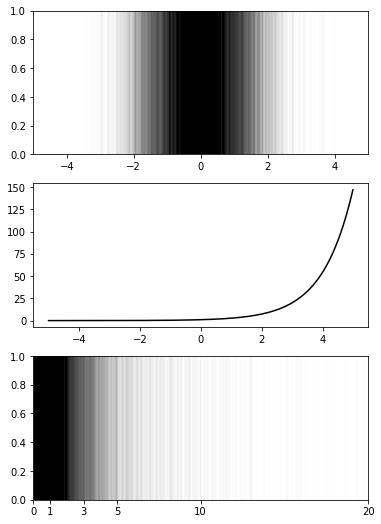
\includegraphics[width=.9\linewidth]{./.ob-jupyter/c59ca9a255316f2f2fb5d2e4cdb6f0a077d97699.png}
\end{center}

After the transformation, the bulk of the probability mass has moved from the center of the real line to the left margin of the positive real line. The saturation of the black lines indicates the concentration of the samples.

\sout{The Standard Normal distribution is of course centered around zero, but the exponential function is certainly not. We can see that all the negative samples in the Normal distribution are squeezed into the \([0, 1]\) region of the resulting LogNormal distribution, and when the quantity is positive, the resulting quantity is stretched to wider and wider regions, because the exponential function is growing faster and faster. This reminds us that probability transformations also distort the distributions, and this distortion consequently affects the property of the new distribution.}

\subsubsection{Logistic transformation}
\label{sec:org585a926}

We can also transform a quantity on \(\mathbb{R}\) to a quantity on \([0, 1]\) using the logistic function

$$y = \frac{1}{1 + e^{-x}} = \frac{e^x}{e^x + 1}.$$

This is a typical sigmoid function, named after the function's S shape:

\begin{verbatim}
x = torch.arange(-5, 5, step=0.01)
plt.plot(x, x.exp() / (1 + x.exp()), 'k')
plt.title('The Logistic function');
\end{verbatim}

\begin{center}
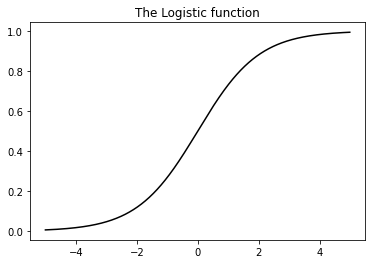
\includegraphics[width=.9\linewidth]{./.ob-jupyter/5551a2c94dbbc7acbbf157b17ae7f259cc299c6c.png}
\end{center}

We can see that the function is symmetric around zero, responsive around \([-4, 4]\), and gradually become less and less responsive when the absolute value is bigger than four. We transforming a distribution we obviously want the resulting distribution to be responsive to the inputs, so we should be attentive where the input values concentrate on.

This time, rather than using a Standard Normal distribution, we will use a Cauchy distribution. This is just to show that we can transform any distribution on \(\mathbb{R}\) in such a way, not only Normals, and certainly not only Standard Normals.

\begin{verbatim}
fig, axes = plt.subplots(2, 1, figsize=(6, 6))

d0 = dist.Cauchy(-1, 2)
x_samples = d0.sample([1000])
y_samples = x_samples.exp() / (1 + x_samples.exp())

sns.histplot(x_samples, ax=axes[0], stat='probability')
axes[0].set_title('Cauchy distribution')
axes[0].set_xlim([-10, 10])
axes[0].set_xticks([-7, -5, -3, -1, 1, 3, 5, 7])

sns.histplot(y_samples, ax=axes[1], stat='probability', bins=50)
axes[1].set_title('Logistic transformed distribution')

plt.tight_layout();
\end{verbatim}

\begin{center}
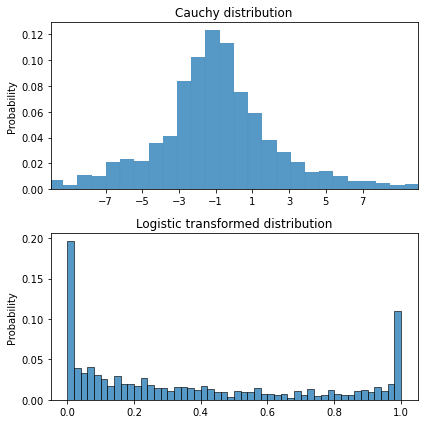
\includegraphics[width=.9\linewidth]{./.ob-jupyter/eebcd9efff12808b2adff3a877a3be9ed25281ee.png}
\end{center}

One striking thing we'd immediately notice is that there are many values close to 0 and 1. This is because in the Cauchy distribution we have many values with absolute values greater than 4, since the logistic function is not responsive to these inputs, all of them are squeezed together after the transformation. It's easier to spot the problem if we colourise the samples:

\begin{verbatim}
fig, axes = plt.subplots(3, 1, figsize=(6, 9))

d0 = dist.Cauchy(0, 2)
x_samples = d0.sample([10000])
y_samples = x_samples.exp() / (1 + x_samples.exp())

for i in range(len(x_samples)):
    x, y = x_samples[i], y_samples[i]
    if x < -4:
        axes[0].axvline(x, color='k', alpha=0.01)
        axes[2].axvline(y, color='k', alpha=0.01)
    elif x < 0:
        axes[0].axvline(x, color='r', alpha=0.01)
        axes[2].axvline(y, color='r', alpha=0.01)
    elif x < 4:
        axes[0].axvline(x, color='k', alpha=0.01)
        axes[2].axvline(y, color='k', alpha=0.01)
    else:
        axes[0].axvline(x, color='r', alpha=0.01)
        axes[2].axvline(y, color='r', alpha=0.01)

axes[0].set_xlim([-10, 10])
axes[0].set_xticks([-8, -4, -1, 4, 8])

x = torch.arange(-5, 5, step=0.01)
axes[1].plot(x, x.exp() / (1 + x.exp()), 'k');
\end{verbatim}

\begin{center}
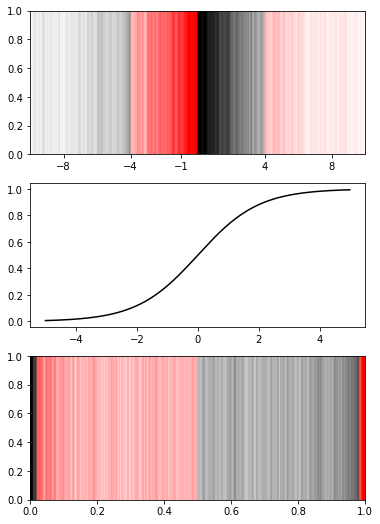
\includegraphics[width=.9\linewidth]{./.ob-jupyter/6f6a16e25fd8b27743bbdc2071af4e35e228b2ba.png}
\end{center}

In this plot we can more clearly see how the transformation distorts the original space. Almost everything left of \(-4\) is squeezed to zero, while everything larger than \(4\) is pushed to one. The middele regions are more equally spreaded but the distortion is also clearly visible. This reminds us that if we want to use the logistic transformation, we probably should first make sure that the original quantity is right in the middle of the real line, between \(-4\) and \(4\). Once beyond, the resulting distribution will stop responding to the input and we are unlikely to learn anything from it. (This, coincidently, is why we have the vanishing gradients problem in many deep learning models.)

\subsubsection{Tailor made transformations}
\label{sec:org66721dd}

Clearly we won't be able to cover all the transformations for probability distributions because the possiblity is literally infinite. The above transformations are all quite important in probabilistic modelling, that's why we have singled them out. But they also serve to demonstrate how to transform probability distributions in general, and the potential pitfalls we should be careful of.

On our probabilistic modelling journey we will encounter many quantities that can, as we reasonably believe, only take on certain values from certain regions of the real line. For example, if we are studying the correlation between two quantities, we know that the correlation can only be between \(-1\) and \(1\); or if we want to study the wight of an apple, we know that it can't possibly exceed several kilograms. These information can help us choose probability distributions for the quantity we are trying to understand. But we have no distributions (not yet at least) on \([-1, 1]\), and if we are modelling the weight of an apple in kilograms, we probably need a distribution on \([0, 10]\), and we don't have that either. So what should we do?

We do what we have already been doing, by transforming known probability distributions on known spaces to the new spaces. If we have already a distribution for some quantity \(x\) on \([0, 1]\), like the Beta distribution, then to define a probability distribution for another quantity \(y\) on \([-1, 1]\) we can simply use the function

$$ y = 2x - 1.$$

We need the scaling coefficient \(2\) because the new space has twice the length as the old one, and we need the translation coefficient \(-1\) because the starting point for the old distribution is \(0\) while the new one is \(-1\). This is quite straightforward.

Likewise to get a distribution for the quantity \(z\) on \([0, 10]\) we can just scale up \(x\)

$$ z = 10 x.$$

There is no need for translation because the two distributions already have the same starting point.

Using this way we can build as many new distributions as we want, and this flexibility is one of the most important strengths of probabilistic modelling. However we should be reminded once again that just because we can construct new distributions however we want, the resulting probability distributions might have properties that surprise us, and come back to bite us if we do not pay enough attention to them.

\subsection{The assemblers}
\label{sec:org22c20f5}

The probability distributions we have studied so far are all simple one dimensional distribution defined on the real line, or a portion of the real line. What if we want to build more sophiscated distributions on higher dimensional spaces?

It turns out that there is a simple rule we can follow to glue simpler distributions together to make distribuitons on higher dimensional spaces, and this rule is called the product rule. Note that it's called a \emph{rule}, something that people follow so that after gluing together different distributions the resulting product is still a distribution; it's not a law or a theorem whose validity has to be proved.

Any way we digressed. The product rule states that the joint probability density of two variables is the product of the density of one variable with the density of the other, conditioned on the value of the first variable, and the rule can be extended to more than two variables. We can write it done as

$$ p(x, y) = p(x) p(y ; x) = p(y) p(x ; y). $$

Here conditioning simply means that when considering the probability of one variable we taken the value of the other variable as given, and we noted it with a semicolon. Tonight, before going to sleep, we comtemplate whether we should carry un umbrella tomorrow morning, just in case it rains; comes the morrow, it is already pouring: this new reality rendering the unbrella problem a totally different problem, because we have to condition on the fact the rain has changed from a possibility to a reality. It turns out that conditioning is the most important concept in modelling and inference, and probably also in life; as such we should treat it with respect and tread carefully when we consider it. Conditioning can change our perception of how things work and what things are, conditioning can also leads to absurdity. We can not condition on the moving air when studying the wind, because the wind is the moving air; we can not condition on the heat when studying the sweating, because sweating is the heat. As much, we should always keep conditioning in mind, but we should also be aware that conditioning is not always sensible.

With this caution in mind, here is how we use conditioning to assemble simpler distributions to build more complex ones. Oh by the way, this practice is normally known as probabilistic modelling.

\subsubsection{A hundred floors above}
\label{sec:org8ef145a}

When we introduced the Bernoulli distribution, we have already been introduced to the endless uncertainties piling up on each other:

\begin{enumerate}
\item We started with a binary quantity, rain or not rain, which has been modeled with a Bounoulli distribution \(\text{Bern} (x; p)\).
\item Since we are not sure about the probability of rain, the quantity \(p\) has been modeled with another distribution, a Beta distribution, because \(p\) can only take values between 0 and 1. The said distribution is \(\text{Beta} (p; a, b)\);
\item The Beta distribution in turn has two more unknown quantities, \(a\) and \(b\), both are unknown postive numbers. We already know several different distributions defined on this space, perhaps we could put a Gamma distribution on one of them and an Exponential distribution on another. That will give us \(\text{Gamma} (a; \alpha, \beta)\) and \(\text{Exp} (b; \lambda)\).
\item Now the new Gamma and Exponential distributions introduced three more unknown quantities, \(\alpha\), \(\beta\), and \(\lambda\). What should we do with them?
\end{enumerate}

At this point we can carry on like before, and model these quantities with new distributions. As the title suggests, we can go directly a hundred floors above the tower and introduces new distributions on each floor. In principle there is nothing stopping us doing that.

Well if the difficulty is not in principle, in practice there are certain limits that we need to consider. Just like if you climb too high the air will grow thinner and thinner and we'd have problem to breath freely, if you build the model with too many layers of uncertainty, in the end the knowledge we have about those newly introduced quantities will grow thinner and thinner and it will resemble more and more random guess. At some point we have to stop climbing begin to enjoy the view.

So if we have decided to go no further, how should we assign values to \(\alpha\), \(\beta\), and \(\lambda\)? At this point there are generally two options:

\begin{itemize}
\item if we have stopped the model building process timely, and we still have some knowledge about what their value should be, then we should assign them values based on this knowledge. This is called the prior information, with "prior" indicating that we already have this knowledge before building this model.
\item if we don't have any reliable information to assign them values, then we should just assign them some values in accordance with common sense. We'll then let the model tell us how well the assignments are, and change them is they turn out to be horrible.
\end{itemize}

The detailed application of these techniques and the art of perfecting them is the main goal of this book.

Now that we already have the conditional distributions for \(x\), \(p\), \(a\) and \(b\), and we have assigned fixed values \(\alpha_0\), \(\beta_0\) and \(\lambda_0\) to the quantities we don't want to model, we can write down the joint density function of \(x\), \(p\) and \(a\) as

$$ p(x, p, a, b; \alpha_0, \beta_0, \lambda_0) =
\text{Bern} (x; p) \text{Beta} (p; a, b) \text{Gamma} (a; \alpha_0, \beta_0) \text{Exp} (b; \lambda_0).$$

Already quite a daunting distribution, isn't it? We'll build far more complex ones later in the book. We see that the distribution of \(x\) is conditioned on \(p\), while \(p\) itself is conditioned on \(a\) and \(b\). \(a\) and \(b\) in turn are conditioned on the values of \(\alpha_0\), \(\beta_0\), and \(\lambda_0\). And the joint density function is just the product of them all.

One more thing worth noticing is that there are actually no distributions that are not conditioned on other quantities, most of the time it's either we are not aware of this conditioning, which amounts to the limitations of our model; or that we are condtioning on fixed values so we don't bother to mention it, just like the fixed parameters for the Gamma and Exponential distributions here.

Right now the unknown quantities form a long chain which ends with one single outcome, but this doesn't need to be the case. The model we are building is for tomorrow's weather, but it doesn't have to limit itself to tomorrow's weather, it can be used for any day in the future; the probability for rain can be different from one day or another, depending on it's winter or summer, tropical area or somewhere near the Arctic. Because of this we can generate, for example, two different probabilities for rain, \(p_1\) and \(p_2\), from the Beta distribution, and using \(p_1\) as the parameter for one Bernoulli distribution that model the weather for three different days \(x1, x2, x3\), while using \(p_2\) for two other days \(x4\) and \(x5\).

So we now have greatly increased the number of quantities we are modelling. But no worry, just apply the simple product rule over and over we'll get where we want.

First for the weather, since the first three days are conditioned on \(p_1\) while the other two on \(p_2\),

\begin{align*}
p(x_1, x_2, x_3, x_4, x_5) &= p(x_1; p_1) p(x_2; p_1) p(x_3; p_1)p(x_4; p_2)p(x_5; p_2) \\
&= \prod_{i=1}^3 p(x_i; p_1) \prod_{i=4}^5 p(x_i; p_2) \\
&= \prod_{i=1}^3 \text{Bern}(x_i; p_1) \prod_{i=4}^5 \text{Bern}(x_i; p_2)
\end{align*}

Then for the probabilities, which we now have two:

\begin{align*}
p(p_1, p_2) &= p(p_1; a, b) p(p_2; a, b) \\
&= \text{Beta} (p_1; a, b)\text{Beta} (p_2; a, b)
\end{align*}

Then adding in the distributions of \(a\) and \(b\), which have stayed the same, we now have a joint density function of

\begin{align*}
& p(x_1, x_2, x_3, x_4, x_5, p_1, p_2, a ,b) \\
&= \prod_{i=1}^3 \text{Bern}(x_i; p_1) \prod_{i=4}^5 \text{Bern}(x_i; p_2) \text{Beta} (p_1; a, b)\text{Beta} (p_2; a, b) \text{Gamma} (a; \alpha_0, \beta_0) \text{Exp} (b; \lambda_0).
\end{align*}

This is a fairly complicated model, and in the future we'll learn to make inference with such models, once we have make some observations. But for now, just observe how we build up complex distributions from simpler ones.

You might be intimedated by the construction of probability density functions for these complex distribution, because it looks like a very error prone practice. But don't worry, nowadays we can normally rely on computer programs to do this for us. The formulae here are just for demonstration and we don't even write out explicitly the probability density functions for each component distribution!

\subsection{Conclusion}
\label{sec:org39bd8c5}

In this chapter we have covered the basics of probability theory, we have introduced some probability distributions, and how to construct new distributions ourselves, and we have showcased how probabilistic modelling is just gradually building up more and more complex joint probability distributions. Clearly we have not covered everything there is to know about probability theory, and we haven't even scratched the tip of the probability distributions iceberg. But that's not the point. What we want to do here is introduce the first principles, both in theory and in practice. We have the rest of the book to expand our knowledge on both regards.

You might be surprised that we haven't even touched on Pyro, the probabilistic modelling language that we plan to use. This is because to do probablistic \textbf{modelling} we actually don't need Pyro, we only need a big enough managerie of probabilistic distributions. It's only when we have observed some data, and we want to do \textbf{inference} on the model we have built, that we actually need it. Pyro has many useful tools and algorithms to do inference on the models we build, and in the next chapter we'll start with one of the most powerful and widely used technique for doing inference on probabilistic models: Markov Chain Monte Carlo.

\section{Probabilistic computation with Markov Chain Monte Carlo}
\label{mcmc}
In chapter 1 we have already built many probabilistic models, and the reader might have been surprised to notice that we haven't used Pyro at all. This is because to do probabilistic \textbf{modelling} we actually don't need any specific probabilistic programming language: all we need is a collection of probability distributions we can build upon, and we then just follow the tree of uncertainty all the way up, as we have done in the last chapter.

However, building distribuitons is one matter, understanding them is quite another. Humans have the habit of creating things that they don't fully understand: Frankenstein's monster is one such example, probability distributions another. Things are relatively manageable if the distribution has only one or two dimensions, we can plot out their density functions and look at how they vary across the space. What should we do if they are of higher dimensions? Three dimensional plots are already difficult to understand, four dimensional or higher are beyond our imagination. When visualising the whole distribution becomes impossible, we settle on ways that we can summarise them.

It turns out that the best way to understand distributions (albeit still limited) is the same as the best way to construct them: by their computational consequences. In the last chapter, through the maximum entropy principle, we have constructed many distributions by forcing them to satisfy certain constraints, notably what their means and variances should be. For example, to build a Normal distribution with \(\mu=2\) and \(\sigma=3\), we construct a probability density function \textbf{so that} the mean can be 2 and the standard deviation can be 3. In other words, when it comes to probability distributions, their essence comes before their existence. In a similiar fashion, to understand higher dimensional distributions we'll also look at their computational consequences, like the mean and variance, and some times maybe also other summary statistics.

Unfortunately getting these summary statistics is also not easy, because there are a large amount of integrations involved. Take as example the Bernoulli-Beta-Gamma distribution we built in last chapter,

$$ p(x, p, a, b; \alpha_0, \beta_0, \lambda_0) =
\text{Bern} (x; p) \text{Beta} (p; a, b) \text{Gamma} (a; \alpha_0, \beta_0) \text{Exp} (b; \lambda_0),$$

to get the mean of \(p\) we'd need to first calculate its marginal distribution, which means marginalising out all the other variables

$$ p(p) = \int p(x, p, a, b; \alpha_0, \beta_0, \lambda_0) dx da db, $$

and then integrate \(p\) over the space of \(p\)

$$ \mathbb{E} (p) = \int p(x) p dp. $$

Both of these two steps are anything but easy, in fact they are extremely difficult, if not outright impossible. As workaround we normally turn to some form of approximations, and one such approximation is to replace these difficult densities with ones similar to them yet easy to compute, so that we can carry out these integrations; this is known as variational inference and will be covered in the next chapter. Another approximation method is to use the samples of these distributions, rather than the densities, to compute the expectations, so that we can reduce the integration problems to mere summations, and that will be the focus of this chapter.

However there are still some extra concerns that need to addressed. There are infinitely many probabilistic models we can build, as shown in the previous chapter, but unfortunately the approximations will only work on some of them. Exactly what models can be built will depend on the probabilistic modelling languages we use, and exactly what models can be learned will depend on the inference algorithms implemented along with the modelling language. Luckily Pyro has a very flexible programming language so that it can express a large amount of very complex models, and the inference engines implemented in Pyro guarenntee that we can learn efficiently from them. Still, it's helpful to remember that like any other modelling and inference package out there, there are limits to what Pyro can do.

\begin{verbatim}
import torch
import torch.distributions as dist
import matplotlib.pyplot as plt
import seaborn as sns
sns.set_theme(palette='Set2')
colors = sns.color_palette()
\end{verbatim}

\subsection{Modelling and Inference in Pyro}
\label{sec:org67d8f9e}

Now let's start with a simple two dimensional Normal distribuiton, and go through the complete Bayesian inference procedure, to see how we can use Pyro for probability modelling and computation. Suppose we have observed the following data:

\begin{verbatim}
mus = torch.tensor([2., 1])
Sigma = torch.tensor([[1, 0.3], [0.3, 0.25]])
mv = dist.multivariate_normal.MultivariateNormal(mus, Sigma)
y = mv.sample([100])
plt.scatter(y[:, 0], y[:, 1])
plt.xticks([0, 2, 4])
plt.yticks([-1, 1, 3])
plt.title("Observed two dimensional data");
\end{verbatim}

The first intuitive reaction, after observing such data, is that we have two variables and the two are correlated; and if you have taken any elementary statistics class, you might be attempted to run a linear regression on it, treating one as an exogeneous variable, i.e. a quantity we observed but not interested in modeling, and another as an endogeneous variable, i.e. what we actually model. It's a valid thing to do, but it treats the two one dimensional variables as separate quantities, here we want to model them jointly, as one two dimensional variable.

How should we build a model for this two dimensional data? We can see that on each dimension the variable can take on continuous values on the whole real line, so two dimensional Normal seems to be a reasonable choice.

Actually what we have just said isn't completely correct, in fact it's totally wrong: we have neither observed any continuous change in the variables, nor have we seen the possible values extending to infinity. None of these two things, continuity or infinity, is actually observable; they only exist in our imagination and are part of the assumptions we've made, unconsciouly. In statistics, as in life, we often make many assumptions that we are ourselves hardly aware of, and it takes active practice and tremendous effort to avoiding doing so. But still, the observed values seems to be real numbers, so we'll pretend they are continuous; and as we have discussed before, once the mean is determined, the Normal distributions only assign non-negligible amount of probability to the region narrowly surrounding the mean, while the exact level of narrowness is determined by the standard deviation. All in all the two dimensional Normal assumption does not sound too outrageous and we will stick to it. So the probability density function for each observed variable can be described as

$$y_n \sim \mathcal{N}(\boldsymbol\mu,\, \boldsymbol\Sigma)$$

in which \(\boldsymbol\mu\) is a vector of means and \(\boldsymbol\Sigma\) is the covariance matrix, we have already met them in the last chapter.

We of course have no idea what their exact values are, and if we want to learn about them we'd have to climb the tower of ignorance and model them one by one. Looking at the plot we have a rough idea what their possible range might be, for example the mean on one direction seems to be around two while on the other direction it's around one, we'll use these values when modelling them.

And how much do they vary? That's a bit more difficult to determine, because remember we are talking about our uncertainty about the means, which is unobservable; not the variations in the data, which we have visualised. However we are at least certain of one thing: the uncertainty in the means shouldn't exceed the variations in the data, since, after all, they are the means of the data.

Finally since they are real values, we can always put a Normal distribution on them. So we can model the means with

\begin{align*}
\mu_{0} &\sim \mathcal{N} (2, 3) \\
\mu_{1} &\sim \mathcal{N} (1, 3)
\end{align*}

As for the standard deviations, they are positive values and we've already known several distributions on this domain, and Gamma seems quite alright.

Other that those we only have the correlation variable left. Normally the correlation between two variables can be anything between -1 and 1, but looking at the plot we are quite sure that the correlation is positive, so that leaves the possible domain to be \([0, 1]\). And for this domain we already have the Beta distribution.

You may have noticed that we have based our priors very tightly on the observed data. There is an old adage in statistics that "you only look at the data once", but that's not the rule we are going to follow here.

One of the main concerns addressed by this adage is that if we look at the data multiple times, we might overfit the data.

Bayes' rule

For example, we can build a two dimensional Gaussian model

Use Markov Chain Monte Carlo to infer the hidden parameters.

look at the recovered parameters

draw samples from them

If you have read some introductory text about Bayesian modelling and inference, it probably only takes less than ten lines of code and one or two paragraphs of explication to cover all we've covered in this section. However, with statistics, like with any other serious subject, examining them a bit more closely always bring us more questions. And since applying statistical methods in real problems always demands close inspections of the problems, more thinking is something we strongly recommend, even though we don't always like doing so.

If this is your first experience with probabilistic modelling and
Bayesian inference, right now you might want to learn more about other
modelling techniques and other algorithms.

How exactly does it work? Carry on.

\subsection{MCMC and the Metropolis-Hastings algorithm}
\label{sec:org365524d}

We have gone through the whole probabilistic computation process with
MCMC method in the previous section, however the whole thing looks a bit
like magic:

\begin{itemize}
\item How exactly are the samples generated?
\item What are the extra values returned by the sampling engine?
\item Can we trust the results the engine is giving us?
\end{itemize}

In this section we'll open the lid and look at the internals of the
sampling engines and see what exactly is going on.

we can easily write out the density function of the two dimensional
Normal distribution

The first model we'll consider is a two dimensional Gaussian, and the
two dimensions are independent of each other. The joint density can be
written out as

\begin{align*} \pi(p) &= \pi(p_{0}) \pi(p_{1}) \ &= \textrm{N} (p_{0};
\mu_{0}, \sigma_{0}) \textrm{N} (p_{1}; \mu_{1}, \sigma_{1}) \ &=
\frac{1}{\sqrt{2 \pi \sigma_{0}^{2}}} \exp { - \frac{1}{2\sigma_{0}^{2}}
(p_{0} - \mu_{0}^{2}) } \frac{1}{\sqrt{2 \pi \sigma_{1}^{2}}} \exp { -
\frac{1}{2\sigma_{1}^{2}} (p_{1} - \mu_{1}^{2}) } \end{align*}

Let's fix the priors \((\mu_{0}, \sigma_{0}) = (1, 1)\) and
\((\mu_{1}, \sigma_{1}) = (-1, 1)\), and the log density therefor is

\begin{align*} \log \pi(p) &= - \frac{1}{2} \log(2 \pi \sigma_{0}^{2}
\sigma_{1}^{2} ) - \frac{(p_{0} - \mu_{0})^{2}}{2 \sigma_{0}^{2}}

- \frac{(p_{1} - \mu_{1})^{2}}{2 \sigma_{1}^{2}} \ &= - \frac{1}{2}
  \log(2 \pi ) - \frac{(p_{0} - 1)^{2}}{2} - \frac{(p_{1} + 1)^{2})}{2}
  \end{align*}

As we can see the log density is always negative, and it's a function of
the values of the variables. In Hamiltonian Monte Carlo we normally use
its negative, which is called the potential function. We can write

the density functions

We can write down the mathematical models, then we transform them
directly into \texttt{logpdf} functions, because that's what really matters in
inference.

Different probabilistic programming languages transform normal computer
code into logpdf functions; if we can write down logpdf functions
directly, then we don't need the intermediate probabilistic programming
languages.

The goal of sampling is to draw from a density \(p(\theta)\) for
parameters \(\theta\). This is typically a Bayesian posterior
\(p(\theta|y)\) given data \(y\), and in particular, a Bayesian posterior
coded as a Stan program.

the logpdf function

a multivariate function

the conditional logpdf function

feed data to the model is fixing some variables

using partial function

In Pyro a model is represented as a computational graph:

And after we have observed some data, we can condition on these
observations. Then the model is updated to a conditional distribution,
with the observed variables' value being fixed to the observed.

Given the conditional distribution, we can now start considering drawing
samples from it.

We have to start some where in the probability space.

initialisation

Then from this initial point, we let the MCMC transition kernel
determine where we'll end up to. There are many different MCMC kernels,
this affects how efficient we can explore the probability space. Here
we'll start with one of the simplest MCMC algorithms, the
Matropolis-Hastings algorithm.

Since the samples are drawn sequentially, we can even follow the samples
trace.

visualise it

This is only a 2D distribution, of course we can easily visualise it.
But we can also look at the marginal distributions are summary
statistics.

And let's see the dynamic progress and how our sampling recover the true
values.

The results looks great, we can look at the marginal distributions.

but can we generalise to more models? This two dimensional Gaussian
model is well behaving, we can see it has only one mode, the density all
concentrates on one point and them gradually decreases. There is on high
curvatures, no multimodes, and no heavy tails.

Let's also try this algorithm on a more demanding model, which is a
funnel distributions with high curvatures.

\subsection{Hamiltonian Monte Carlo}
\label{sec:org2d034ee}
HMC is an auxiliary MCMC method.

Hamiltonian Monte Carlo (HMC) is a Markov chain Monte Carlo (MCMC)
method that uses the derivatives of the density function being sampled
to generate efficient transitions spanning the posterior (see, e.g.,
@Betancourt-Girolami:2013, @Neal:2011 for more details). It uses an
approximate Hamiltonian dynamics simulation based on numerical
integration which is then corrected by performing a Metropolis
acceptance step.

HMC introduces auxiliary momentum variables \(\rho\) and draws from a
joint density

$$
p(\rho, \theta) = p(\rho | \theta) p(\theta).
$$

In most applications of HMC, including Stan, the auxiliary density is a
multivariate normal that does not depend on the parameters \(\theta\),

$$
\rho \sim \mathsf{MultiNormal}(0, M).
$$

\(M\) is the Euclidean metric. It can be seen as a transform of parameter
space that makes sampling more efficient; see @Betancourt:2017 for
details.

By default Stan sets \(M^{-1}\) equal to a diagonal estimate of the
covariance computed during warmup. the potential is the negative log
pdf.

\subsubsection{The Hamiltonians}
\label{the-hamiltonians}
We saw that when the dimension of a distribution is high, or when the
target density function is not very smooth, the Metropolis algorithm can
be very inefficient, since most of the proposals will be rejected, and
the sampler is stuck at one region of the sampling space, unable to
explore the whole space efficiently.

This prompts us to look for other MCMC methods that are less random and
consequentially more efficient. The method we are going to cover here is
Hamiltonian Monte Carlo, and it's based on two important ideas:

\begin{itemize}
\item Sometimes it might be difficult to sample from the target distribution
but it can be easier to sample from a higher dimensional distribution,
of which the target distribution is its marginal distribution. This
might sound counter-intuitive but there are actually a family of
Markov Chain Monte Carlo methods that make use of this idea, Slice
sampling is one of them, and the Hamiltonian Monte Carlo algorithm we
are covering here is another. The reason for this counter-intuitive
behaviour, is that the higher dimensional distribution might have some
extra structure that we can use to facilitate the sampling.
\item If we limit the family of distribution we are sampling from, we might
be able to devise some more efficient sampling methods for this
limited family of distributions. With Hamiltonian Monte Carlo we want
to use the derivative information of the target density. This limits
the kind of distributions we can sample from, since only continuous
distributions have densities. (However, all is not lost. For many
joint distributions in which some of the variables are discrete, we
can first integrate out the discrete variables, then sample the
continuous variables using Hamiltonian Monte Carlo.)
\end{itemize}

Here we'll first introduce what is the Hamiltonian, then how to
construct the Hamiltonian, and finally how to sample from it.

\subsubsection{Initialising the sampler}
\label{initialising-the-sampler}

\subsection{Sampling the Hamiltonian with \texttt{NUTS}}
\label{sec:orgdf1211f}
Mixture of Gaussians

\begin{align*} y_n &\sim \text{Normal}(\mu_{z}, , 1) \ z_{n} &\sim
\text{Bernoulli}(0.7) \ \mu_{k} &\sim \text{Normal}(0, 2). \end{align*}

neural networks, mixture models.

transitioning between the modes is difficult; it contradicts the basic
goal of MCMC.

with MCMC we want to move to regions of high probability; to move from
one mode to another, we need to first move away from one mode, then move
to another mode.

\subsection{Some other sampling methods}
\label{sec:org824dca6}

\subsection{Closing thought}
\label{sec:orgdba570c}
\end{document}
